% =====================================================================
% Revised version of the author's hand-written ThesisProj draft.
%
% The author's sentences are kept wherever the review did not require a
% change. Everything added or edited is marked in the margin of this source
% with  % [NEW]  or  % [EDIT]  so the two can be told apart at a glance.
%
% What changed and why (full detail: reports/p22/review_response_paperA.md):
%   [EDIT] Eq. (9) had no left-hand side. Added Y.
%   [EDIT] Sec. IV-A used q and y for the same imaginary part. Now y throughout.
%   [EDIT] Sec. III-B called (18) a projection. It is not: it is not even
%          idempotent. Rewritten honestly, with a worked number.
%   [EDIT] Sec. III-C said 70% of the pilots estimate the channel. The code
%          refits on ALL pilots after the rank is chosen. Corrected -- this is
%          what makes the comparison against EM-GS fair.
%   [NEW]  Sec. II states the path-gain normalisation, so the path-count sweep
%          is at fixed received power.
%   [NEW]  Sec. II states that this is one Rydberg architecture, not the family.
%   [NEW]  Sec. V-F names the second channel distribution.
%   [NEW]  Sec. IV-B says what the CCRB curve does and does not specify.
% =====================================================================
\documentclass[journal]{IEEEtran}
\IEEEoverridecommandlockouts

\usepackage{amsmath,amssymb,amsfonts}
\usepackage{graphicx}
\usepackage{booktabs}
\usepackage{url}
\usepackage{tikz}
\usetikzlibrary{arrows.meta,positioning}

\DeclareMathOperator{\rank}{rank}
\newcommand{\bG}{\mathbf{G}}
\newcommand{\bS}{\mathbf{S}}
\newcommand{\bB}{\mathbf{B}}
\newcommand{\bW}{\mathbf{W}}
\newcommand{\bY}{\mathbf{Y}}
\newcommand{\bZ}{\mathbf{Z}}
\newcommand{\bg}{\mathbf{g}}
\newcommand{\CN}{\mathcal{CN}}
\newcommand{\Hank}{\mathcal{H}}
\newcommand{\rmax}{r_{\mathrm{max}}}
\newcommand{\reff}{r_{\mathrm{eff}}}
\newcommand{\ncz}{n_{\mathrm{cz}}}
\newcommand{\dhs}{\Delta_{\mathrm{HS}}}

\begin{document}

\title{Hankel-Structured Channel Estimation for\\
Magnitude-Only Rydberg Atomic Receivers:\\
When Does Structure Help?}

\author{Abdullah~Haatim%
\thanks{A.~Haatim is with the Department of Electrical and Electronics
Engineering, Birla Institute of Technology and Science, Pilani~--- Pilani
Campus, India (e-mail: f20220519@pilani.bits-pilani.ac.in).}}

\maketitle

\begin{abstract}
We study channel estimation for a magnitude-only Rydberg atomic receiver array,
in which the optical readout provides the amplitude of the incident
radio-frequency field but not its phase, so complex channel estimation becomes
a phase-retrieval problem. Rydberg architectures that recover phase, such as a
superheterodyne readout, are outside this scope. This paper asks when the known
spatial structure of a multipath channel improves such magnitude-only
estimation, and when that structure is too restrictive to help. We propose a
Hankel-structured extension of expectation--maximization Gerchberg--Saxton
(EM-GS) that exploits the relationship between channel coefficients across a
uniform linear array, choosing the amount of structure from held-out pilot
measurements. Selecting the full rank disables the structural step, and the
estimator then returns the EM-GS answer exactly; this is a property of the
operator and not a guarantee that the selection rule avoids harmful choices.
Simulations show that the structural step helps when the channel is simple
relative to the structural capacity of the array, and that its benefit falls,
and eventually reverses, as channel complexity approaches that capacity. In a
held-out comparison, path count normalized by that capacity predicts the
measured gain far better than path count alone, and the prediction transfers to
two channel distributions not used to build it. A constrained Cram\'er--Rao
bound for the multipath model, derived and verified here, quantifies what the
structure is worth in principle. These results give a practical account of when
spatial structure should be exploited in magnitude-only channel estimation and
when an estimator should rely on the unconstrained solution instead.
\end{abstract}

\begin{IEEEkeywords}
Rydberg atomic receiver, channel estimation, phase retrieval, Hankel matrix,
constrained Cram\'er--Rao bound, effective rank.
\end{IEEEkeywords}

\section{Introduction}

\IEEEPARstart{S}{ixth-generation} wireless systems are expected to operate over
wider bandwidths and at increasingly high carrier frequencies, placing new
demands on receiver sensitivity and reconfigurability. Quantum sensing has
emerged as one possible response, and Rydberg atomic receivers have recently
attracted attention for wireless communications~\cite{cui2025,gong2025mag}.
These receivers use laser-excited atoms to sense an incident radio-frequency
field through changes in optical transmission. Unlike a conventional coherent
receiver, however, the optical readout directly provides the field amplitude
rather than its complex value, so the channel phase is not directly observed.

Recovering a complex channel from these amplitude-only measurements is a
phase-retrieval problem. A known reference field makes this recovery possible
by converting relative phase into observable amplitude. Existing approaches
include iterative phase-retrieval methods~\cite{gerchberg1972}, gradient
descent with structural projection~\cite{xu2025}, and unrolled
networks~\cite{xiao2026}. These works focus mainly on improving channel
estimation performance. Less attention has been given to a more basic question:
when does imposing channel structure actually help, and when does that
structure become too restrictive? This paper addresses that question using the
spatial structure of multipath channels on a uniform linear array.

We propose a Hankel-structured extension of EM-GS for magnitude-only channel
estimation. The estimator exploits the exponential structure of the channel
across the array, selects the structural order using held-out pilot
measurements. When the selection returns the full rank the structural step
changes nothing and the estimator reproduces EM-GS exactly; this is a property
of the operator, and it is not a guarantee that the selection rule avoids
choices that hurt. We then study how the benefit of the Hankel
constraint changes with the array size and the complexity of the channel. Path
count alone does not fully describe channel complexity, so we also describe
channel complexity using its effective rank relative to the available Hankel
rank. Finally, we test this relationship on two additional channel
distributions.

\section{System Model}

We consider an uplink system with $K$ single-antenna users and one Rydberg
atomic receiver, as shown in Fig.~\ref{fig:system}. The receiver contains $N$
vapour-cell receive elements arranged in a uniform linear array (ULA). Each
vapour cell contains atoms that are excited to Rydberg states using probe and
coupling lasers. The RF signals transmitted by the users interact with these
atoms. A known RF reference field is also applied at the receiver. The atomic
response changes the probe laser passing through the vapour cell, and this
change is measured using a photodetector. The receiver therefore measures the
strength of the total RF field, but it does not directly observe its complex
phase~\cite{cui2025}.

% [NEW] Physical scope. The review asked for this: the paper studies one
% architecture, not every Rydberg receiver.
\textbf{This paper studies one Rydberg architecture, not all of them.} There
are Rydberg receivers that use a superheterodyne readout, in which a local
reference drives the vapour cell and the beat note is detected. Those receivers
recover both amplitude and phase, so the problem studied here does not arise
for them. Everything below applies to the magnitude-only readout described
above. In fact, nothing below depends on the atomic physics itself: the results
apply to any array receiver that measures only the magnitude of the total
field, and the Rydberg receiver is the motivating example.

\begin{figure*}[!t]
\centering
\resizebox{0.86\textwidth}{!}{% System-model figure for Paper 1, Section II.
%
% Convention checked against the reference material in the project directory
% before drawing:
%   * SystemModel.pdf (this project's own model document) -- the terminology
%     "receive element = one vapour cell interrogated by one photodetector",
%     the probe/coupling laser pair, and the signal chain
%     h -> E = GS+B+W -> Omega = |E| -> Delta f -> Z.
%   * Cui, Zeng and Huang, "Towards atomic MIMO receivers" -- users left,
%     atomic array right, reference field drawn as a separate incident beam.
%   * Xu et al., "Channel estimation for Rydberg atomic receivers" -- pilots
%     labelled on the uplink arrows.
%   * Gong et al. survey -- level of physical detail: the vapour cell and the
%     two lasers appear, the energy-level diagram does not.
%
% Deliberately NOT drawn: atomic level structure, Autler-Townes lineshapes,
% optical bench detail. The figure exists to show where the phase is lost.
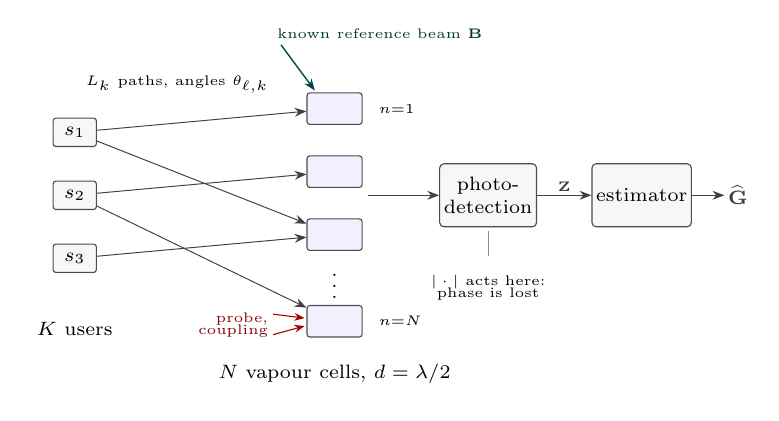
\begin{tikzpicture}[
  font=\scriptsize,
  cell/.style={draw=black!70, fill=blue!6, rounded corners=1pt,
               minimum width=7mm, minimum height=4mm, inner sep=1pt},
  usr/.style={draw=black!70, fill=black!3, rounded corners=1pt,
              minimum width=5.5mm, minimum height=3.6mm, inner sep=1pt},
  blk/.style={draw=black!70, fill=black!3, rounded corners=1.5pt,
              minimum width=12mm, minimum height=8mm, align=center,
              inner sep=1.5pt},
  sig/.style={-{Stealth[length=1.5mm]}, black!75, line width=0.35pt},
  laser/.style={-{Stealth[length=1.3mm]}, red!65!black, line width=0.4pt},
  ref/.style={-{Stealth[length=1.5mm]}, teal!55!black, line width=0.5pt},
]

% ---------------- users -------------------------------------------------
\foreach \i/\y in {1/1.35, 2/0.55, 3/-0.25} {
  \node[usr] (u\i) at (0, \y) {$s_{\i}$};
}
\node[font=\scriptsize, align=center] at (0, -1.15) {$K$ users};

% ---------------- array -------------------------------------------------
\foreach \i/\y in {1/1.65, 2/0.85, 3/0.05, 4/-1.05} {
  \node[cell] (c\i) at (3.30, \y) {};
}
\node[font=\scriptsize] at (3.30, -0.50) {$\vdots$};
\node[right=0.8mm of c1, font=\tiny] {$n{=}1$};
\node[right=0.8mm of c4, font=\tiny] {$n{=}N$};
\node[font=\scriptsize, align=center] at (3.30, -1.72)
  {$N$ vapour cells, $d=\lambda/2$};

% ---------------- propagation -------------------------------------------
\draw[sig] (u1) -- (c1);
\draw[sig] (u1) -- (c3);
\draw[sig] (u2) -- (c2);
\draw[sig] (u2) -- (c4);
\draw[sig] (u3) -- (c3);
\node[font=\tiny, inner sep=0.5pt] at (1.30, 1.96)
  {$L_k$ paths, angles $\theta_{\ell,k}$};

% ---------------- reference beam ----------------------------------------
\draw[ref] (2.62, 2.46) -- (3.05, 1.88);
\node[font=\tiny, teal!45!black, anchor=west, inner sep=0.5pt]
  at (2.55, 2.60) {known reference beam $\mathbf{B}$};

% ---------------- probe and coupling lasers -----------------------------
\draw[laser] (2.52, -0.96) -- (2.92, -1.01);
\draw[laser] (2.52, -1.22) -- (2.92, -1.11);
\node[font=\tiny, red!55!black, anchor=east, align=right, inner sep=0.5pt]
  at (2.48, -1.10) {probe,\\[-1.5pt]coupling};

% ---------------- readout and estimator ---------------------------------
\node[blk] (pd) at (5.25, 0.55) {photo-\\detection};
\node[blk] (est) at (7.20, 0.55) {estimator};

\draw[sig] (3.72, 0.55) -- (pd);
\draw[sig] (pd) -- node[above, font=\tiny, inner sep=1.2pt] {$\mathbf{Z}$} (est);
\draw[sig] (est) -- ++(1.05, 0)
  node[right, font=\scriptsize, inner sep=1.2pt] {$\widehat{\mathbf{G}}$};

\node[font=\tiny, align=center, inner sep=1pt] at (5.25, -0.62)
  {$|\cdot|$ acts here:\\[-1.5pt]phase is lost};
\draw[black!45, line width=0.3pt] (5.25, -0.22) -- (5.25, 0.10);

\end{tikzpicture}
}
\caption{Uplink of the Rydberg atomic receiver. $K$ single-antenna users
transmit known pilot signals to $N$ vapour-cell receive elements arranged as a
uniform linear array. The user RF signals and a known reference RF field
interact with the Rydberg atoms. Probe and coupling lasers are used for the
atomic readout, and the photodetector measures the magnitude of the total
field. The estimator therefore observes $\bZ$ without directly observing its
phase.}
\label{fig:system}
\end{figure*}

We model the channel between each user and the array using several propagation
paths. A path may represent a signal arriving directly from the user or after
interacting with objects in the environment. For user $k$, the channel
coefficient at the $n$th receive element is
\begin{equation}
g_k[n]=\sum_{\ell=1}^{L_k}\alpha_{\ell,k}e^{-j(n-1)\psi_{\ell,k}},\qquad
\psi_{\ell,k}=\pi\sin\theta_{\ell,k},
\label{eq:chan}
\end{equation}
where $L_k$ is the number of propagation paths for user $k$, $\alpha_{\ell,k}$
is the complex gain of path $\ell$, and $\theta_{\ell,k}$ is its angle of
arrival. In our simulations, $L_k$ is selected between 3 and 7, following the
channel setting in~\cite{xu2025}.

The exponential term in \eqref{eq:chan} describes how the phase of one
propagation path changes as we move from one array element to the next. To see
this, consider a single path arriving at the array from an angle $\theta$. The
signal reaches the different array elements at slightly different times because
the elements are at different positions. This difference in travel distance
produces a phase difference between adjacent elements.

With half-wavelength spacing between the array elements, the phase change
between two neighbouring elements is
\begin{equation}
\psi=\pi\sin\theta.
\end{equation}

The first array element has no additional phase shift from the array position.
The second element has a phase shift of $\psi$, the third has a phase shift of
$2\psi$, and so on. Therefore, the samples produced by one path across the
array have the form
\begin{equation}
1,\qquad e^{-j\psi},\qquad e^{-j2\psi},\qquad\ldots,\qquad e^{-j(N-1)\psi}.
\end{equation}

The factor
\begin{equation}
e^{-j(n-1)\psi_{\ell,k}}
\end{equation}
in \eqref{eq:chan} represents exactly this phase pattern for path $\ell$. The
coefficient $\alpha_{\ell,k}$ determines the strength and initial phase of that
path. Since several paths can arrive at the receiver, their contributions are
added together to produce the final channel coefficient $g_k[n]$.

The channel coefficients of user $k$ are collected into the vector
\begin{equation}
\bg_k=\begin{bmatrix}g_k[1]&g_k[2]&\cdots&g_k[N]\end{bmatrix}^T,
\end{equation}
and the channels of all $K$ users are collected into
\begin{equation}
\bG=\begin{bmatrix}\bg_1&\bg_2&\cdots&\bg_K\end{bmatrix}\in\mathbb{C}^{N\times K}.
\end{equation}

During channel estimation, the $K$ users transmit $P$ known pilot symbols.
These pilots are collected in
\begin{equation}
\bS\in\mathbb{C}^{K\times P}.
\end{equation}

Each row of $\bS$ contains the pilots transmitted by one user, while each
column represents one pilot transmission. The same pilot matrix is used when
comparing the different channel estimators.

If the receiver could observe the complete complex signal, the contribution
from the users would be $\bG\bS$. However, the Rydberg receiver considered here
measures magnitude rather than directly measuring this complex value. A known
reference RF field is therefore applied at the receiver. We denote this
reference by
\begin{equation}
\bB\in\mathbb{C}^{N\times P}.
\end{equation}

The reference field is known in both amplitude and phase. It is important
because the magnitude of an unknown signal alone does not directly reveal its
phase. When the unknown user signal is combined with a known reference, the
resulting magnitude depends on their relative phase. This provides information
that can be used to estimate the complex channel.

% [EDIT] Equation (9) had no left-hand side in the draft.
Including noise, the field before the magnitude measurement is
\begin{equation}
\bY=\bG\bS+\bB+\bW,
\end{equation}
where the noise is modeled as complex Gaussian,
\begin{equation}
\bW_{np}\sim\CN(0,\sigma^2).
\end{equation}

The noise is therefore added before the magnitude is measured. The Rydberg
receiver observes
\begin{equation}
\bZ=\left|\bG\bS+\bB+\bW\right|,
\label{eq:obs}
\end{equation}
where $|\cdot|$ is applied to every element of the matrix.

Equation \eqref{eq:obs} is the main measurement model used in this work. The
pilots $\bS$ and reference field $\bB$ are known, and the receiver measures
$\bZ$. The unknown quantity is the complex channel matrix $\bG$. The
channel-estimation problem is therefore to recover $\bG$ even though the
receiver does not directly observe the phase of the received signal.

We assume a narrowband, frequency-flat channel during the pilot interval. The
path gains are modeled as independent circularly symmetric complex Gaussian
variables, and the angles of arrival are independently generated over
$(-90^\circ,90^\circ)$. The users have equal received power, and the reference
field remains known at the receiver. For a fair comparison, all estimators use
the same channel, pilots, reference field, and noise realization within each
Monte Carlo trial.

% [NEW] Path-gain normalisation. The review asked whether total power changes
% when L changes. It does not, and the paper did not say so.
\textbf{The path gains are scaled so that the total received power does not
change with the number of paths.} We draw
\begin{equation}
\alpha_{\ell,k}\sim\CN\!\left(0,\ \beta_k/L_k\right),
\label{eq:pathnorm}
\end{equation}
so that the powers of the individual paths add up to
\begin{equation}
\sum_{\ell=1}^{L_k}\mathbb{E}\left|\alpha_{\ell,k}\right|^2=\beta_k,
\end{equation}
which does not depend on $L_k$. This matters wherever the number of paths is
varied. Without this scaling, adding more paths would also add more received
power, and we could not tell whether a change in performance came from the
extra complexity or simply
from the extra power. With this scaling, only the complexity changes.

The reference-to-signal ratio (RSR) is the reference power divided by the
single-user received signal power. The signal-to-noise ratio (SNR) is the
single-user received signal power divided by $\sigma^2$.

\section{Proposed Estimator}

\subsection{Structure and its Capacity}

The rank of a matrix tells us how many independent components are needed to
describe it. A low-rank matrix is therefore described using only a small number
of important components. To use this idea for our channel, we first rewrite the
channel into a Hankel matrix. A Hankel matrix is a matrix in which the same
channel samples are repeated along the antidiagonals. For example, consider
\begin{equation}
\bg=\begin{bmatrix}g_1&g_2&g_3&g_4&g_5\end{bmatrix}^T.
\end{equation}

One possible Hankel representation is
\begin{equation}
\Hank(\bg)=\begin{bmatrix}
g_1&g_2&g_3\\
g_2&g_3&g_4\\
g_3&g_4&g_5
\end{bmatrix}.
\end{equation}

We use this representation because the channel in \eqref{eq:chan} is not a
random collection of values. It is made up of propagation paths, and each path
produces a complex exponential pattern across the array elements. When this
type of channel is written as a Hankel matrix, each path contributes one
rank-one component. For example, a channel containing one path produces a
Hankel matrix with rank at most one. Two paths produce a matrix with rank at
most two. In general, for a channel with $L_k$ paths,
\begin{equation}
\rank\Hank_p(\bg_k)\le L_k.
\end{equation}

Therefore, when the channel has only a few paths, its Hankel matrix can have a
low rank~\cite{cadzow1988,markovsky2008}. This is why we use the Hankel
representation: it changes the multipath structure of the channel into a
low-rank matrix structure that can be used during channel estimation.

One point of care. The bound is on the number of paths, not on the number of
\emph{strong} paths. A channel with three strong paths and five weak ones has
Hankel rank at most 8, not 3; the weak paths still contribute rank-one
components, however small their singular values. Such a channel is
\emph{approximately} low rank rather than exactly low rank. The distinction
matters, because a rank bound counts paths while the usefulness of the
constraint depends on how many of them carry real energy.

The maximum possible rank of the Hankel matrix depends on the number of array
elements. For an $(N-p)\times(p+1)$ Hankel matrix, the maximum rank is
\begin{equation}
\min(N-p,\,p+1).
\end{equation}

Choosing $p$ so that the matrix is as balanced as possible gives
\begin{equation}
\rmax(N)=\left\lceil\frac{N}{2}\right\rceil.
\label{eq:rmax}
\end{equation}

For example, if $N=16$, the maximum Hankel rank is 8. If the channel has only
three paths, its Hankel rank can be at most 3. This is much smaller
than the maximum rank of 8, so there is useful low-rank structure that can be
used during estimation. If the channel rank is already close to 8, there is
less low-rank structure available. In this case, forcing the channel to have a
much smaller rank may remove part of the real channel.

\subsection{The Baseline: EM-GS}
\label{sec:emgs}

Our starting point is the expectation--maximization Gerchberg--Saxton
estimator, which we call EM-GS, given by Cui \emph{et al.}~\cite[Alg.~2]{cui2025}
as an adaptation of the classical Gerchberg--Saxton
iteration~\cite{gerchberg1972} to this receiver. Because the whole paper is a
comparison against it, it is worth writing down.

The difficulty is that we measure $\bZ=|\bG\bS+\bB+\bW|$ and the phase is
missing. If we knew the phase, the problem would be ordinary linear estimation.
EM-GS therefore alternates between guessing the phase and solving the linear
problem that the guess implies.

Let $\hat\bG^{(t)}$ be the channel estimate after $t$ iterations, and let
$\boldsymbol\Lambda^{(t)}=\hat\bG^{(t)}\bS+\bB$ be the noiseless field it
predicts. One iteration is two steps.

\emph{Expectation step.} Give every measured magnitude the phase that the
current estimate predicts for it, producing a complex field
\begin{equation}
\bY^{(t)}_{np}
=\bZ_{np}\,R(\kappa_{np})\,
\frac{\boldsymbol\Lambda^{(t)}_{np}}{\bigl|\boldsymbol\Lambda^{(t)}_{np}\bigr|},
\qquad
\kappa_{np}=\frac{2\bZ_{np}\bigl|\boldsymbol\Lambda^{(t)}_{np}\bigr|}{\sigma^2},
\label{eq:emgs_phase}
\end{equation}
where $R(x)=I_1(x)/I_0(x)$ is the same Bessel ratio that appears in the Rician
model. This is the conditional mean of the noiseless field given the
measurement and the current estimate, which is what makes the step an
expectation step rather than a plain phase substitution. Because $R(x)<1$, the
imputed field is \emph{shrunk} towards zero relative to the measurement, and
the shrinkage is strongest where the measurement is least informative. At high
SNR $R\to1$ and \eqref{eq:emgs_phase} reduces to substituting the predicted
phase and keeping the measured magnitude.

\emph{Maximization step.} Treat $\bY^{(t)}$ as if it were an observed complex
measurement and solve the resulting least-squares problem,
\begin{equation}
\hat\bG^{(t+1)}
=\bigl(\bY^{(t)}-\bB\bigr)\bS^{H}
\bigl(\bS\bS^{H}+\varepsilon\mathbf{I}\bigr)^{-1},
\label{eq:emgs_ls}
\end{equation}
with a ridge $\varepsilon$ that is set to zero in all experiments here and is
retained only to guard against a singular pilot Gram matrix.

The iteration is started from the spectral initializer of~\cite{cui2025},
computed independently for each receive element, and not from zero. It then
runs for a fixed budget of $T$ iterations rather than to a convergence
tolerance, with $T$ fixed per configuration and stated with the simulation
settings. A fixed
budget is used because it makes the comparison between estimators exact: both
arms get the same number of iterations, so no difference between them can come
from one being allowed to run longer. It also means neither arm is claimed to
have converged.

Nothing in \eqref{eq:emgs_phase} or \eqref{eq:emgs_ls} knows that the channel
comes from a small number of propagation paths. Each channel coefficient is
treated as a free complex number.

\subsection{The Estimator}
\label{sec:estimator}

EM-GS does not follow the rank structure discussed earlier. To include that
structure, we apply a Cadzow denoising step to the channel estimate. There are
three parts to the step. First, the channel estimate is converted into the
Hankel matrix described earlier.

Next, singular value decomposition (SVD) is applied to the Hankel matrix. SVD
separates the matrix into components and gives a singular value for each
component. A larger singular value means that the component has a larger
contribution to the matrix. For example, suppose the singular values are
\begin{equation}
\sigma_1=10,\qquad\sigma_2=6,\qquad\sigma_3=0.3.
\end{equation}

Here, the three singular values are 10, 6, and 0.3. If we decide to use a rank
of 2, we keep the two largest components, corresponding to 10 and 6, and remove
the smaller component corresponding to 0.3. The resulting matrix therefore has
rank 2. If the true channel has only two important components, the removed
component may mainly come from noise or estimation error.

After the rank reduction, the matrix is converted back into a channel vector.
The entries along each antidiagonal are averaged because they represent the
same channel sample. These steps can be written as
\begin{equation}
\mathcal{P}_r(\bg)=\Hank_p^{\dagger}\left(\Pi_r\left(\Hank_p(\bg)\right)\right),
\label{eq:cadzow}
\end{equation}
where $\Pi_r$ keeps the $r$ largest singular values and $\Hank_p^{\dagger}$
converts the Hankel matrix back into a channel vector by averaging its
antidiagonals.

% [EDIT] The draft called this a projection. It is not one, and the review was
% right to flag it. Written out here in the same style as the rest.
\textbf{This step is a denoising step, not a projection.} It is worth being
careful about the word, because the two are not the same thing. A projection
must land on the set it is projecting onto, and applying it a second time must
change nothing. The map in \eqref{eq:cadzow} does neither. Rank reduction
generally destroys the Hankel pattern, and averaging the antidiagonals to
restore that pattern generally raises the rank again.

A small example makes this concrete. Take
\begin{equation}
\bg=\begin{bmatrix}1&2&3&4&5\end{bmatrix}^T
\end{equation}
and use the $3\times3$ Hankel matrix above. Applying \eqref{eq:cadzow} once
with $r=1$ and forming the Hankel matrix of the result gives singular values
\begin{equation}
\left[9.6194,\quad 0.1295,\quad 0.0616\right],
\end{equation}
which is a matrix of rank 3, not rank 1. Applying the same step a second time
moves the answer again, by about $0.099$ in Euclidean distance. A projection
would not have moved it at all. We therefore call \eqref{eq:cadzow} a Cadzow
step~\cite{cadzow1988}, and we apply it repeatedly rather than once, so that
the number of sweeps is part of the definition of the operator. Even when
repeated sweeps settle down, they are not guaranteed to reach the closest
matrix that is both Hankel and low rank~\cite{markovsky2008}.

\textbf{A low Hankel rank is also a weaker requirement than our channel
model.} Equation \eqref{eq:chan} says the channel is a sum of exponentials
whose modes lie on the unit circle, because $e^{-j(n-1)\psi}$ always has
magnitude one. A low-rank Hankel matrix only says the channel is a sum of a few
exponentials; their modes may grow or decay across the array and need not be
angles of arrival at all. Imposing low Hankel rank is therefore a relaxation of
the array model, not the array model itself. We use it because it is easy to
impose and because the true channel does satisfy it, but the constraint is
looser than the physics.

We call the resulting method Hankel-structured EM-GS (HS-GS).

\textbf{Where the step is applied, precisely.} HS-GS applies the Cadzow step
\eqref{eq:cadzow} to each column of the channel estimate \emph{after every one
of the $T$ EM-GS updates}, not once at the end. So a single HS-GS iteration is
the expectation step \eqref{eq:emgs_phase}, the least-squares step
\eqref{eq:emgs_ls}, and then the structural step, in that order, with the
result of the structural step becoming the estimate the next expectation step
predicts from. This matters because the two orderings do not produce the same
answer: denoising an estimate and then iterating is not the same operation as
iterating and then denoising once, and neither is a special case of the other.
The alternative --- running EM-GS to its full budget and applying one Cadzow
step to the result --- is a different and cheaper estimator, and it is measured
separately among the numerical results rather than treated as interchangeable
with this one.

Choosing $r$ is important because a rank that is too large may remove very
little, while a rank that is too small may remove useful parts of the channel.

\subsection{Choosing the Hankel Rank}

The Cadzow step requires us to choose the rank $r$. However, the correct rank
is not known at the receiver, so we choose it using the pilot measurements.

% [EDIT] The draft said the remaining 70 per cent are used to estimate the
% channel. The implementation refits on ALL pilots once the rank is chosen,
% and that is what makes the comparison against EM-GS fair.
The selection is done in two stages, and it is worth separating them clearly.

\emph{Stage one, choosing the rank.} We set aside $30\%$ of the pilot columns.
For each possible rank,
\begin{equation}
r\in\{1,2,\ldots,\rmax\},
\end{equation}
we estimate the channel using only the other $70\%$, and then use that estimate
to predict the magnitude measurements of the held-out pilots. We compare these
predicted magnitudes with the actual measurements. The rank with the smallest
difference, or residual, is selected. For example, if 30 pilots are available,
about 21 are used for these trial estimates and 9 are kept for scoring them.

\emph{Stage two, the final estimate.} Once the rank $\hat r$ has been chosen,
the estimate is computed again using \emph{all} $P$ pilot columns, not only the
$70\%$. The split is used for scoring, and nothing else.

This distinction matters for a fair comparison. HS-GS and EM-GS therefore use
exactly the same number of pilots to produce their final estimates, and the
difference between them is only the Cadzow step. It also means that when the
step is switched off, HS-GS returns exactly the EM-GS answer: in our
simulations the two agree to $\max|\text{diff}|=0$, so the Cadzow step is
provably the only difference between them.

We cannot score the candidate ranks using the pilots that were used to fit
them. Constraining the channel can only make the fit to those pilots worse, so
an in-sample score would always prefer the largest rank, which is the same as
using no constraint at all. Scoring on pilots that were held out penalises
over-modelling correctly.

For example, suppose $\rmax=8$. We test ranks from 1 to 8. If $r=3$ gives the
smallest error on the held-out pilots, we choose
\begin{equation}
\hat r=3.
\end{equation}

We then keep the three strongest singular-value components in the Cadzow step.

This method does not require the true number of propagation paths $L_k$. If the
selected rank is $\rmax$, all singular-value components are kept, the Cadzow
step does not lower the rank, and HS-GS returns exactly the EM-GS estimate.

It is worth being exact about what that does and does not promise. It says the
estimator has a harmless setting available, and that selecting it costs
nothing. It does \emph{not} say the selection rule will choose that setting
whenever the constraint would hurt. The rule scores candidate ranks on held-out
pilots, and a rank that scores well there can still damage the estimate, so a
selected rank below $\rmax$ is not evidence that constraining was the right
choice on that trial.

\section{Performance References}

\subsection{Information in an Amplitude Measurement}

The Cram\'er--Rao lower bound (CRLB) is used as a theoretical reference for
channel estimation. In simple terms, it tells us how accurately an unbiased
estimator could estimate the channel from the available measurements. The
amount of information contained in the measurements therefore affects the CRLB.

This is important for the Rydberg receiver because it measures only the
amplitude of the received signal, not its full complex value. For example,
suppose the noiseless received signal is
\begin{equation}
s=3+j4.
\end{equation}

A complex receiver can observe both the real part, 3, and the imaginary part,
4. The amplitude-only receiver instead observes
\begin{equation}
|s|=\sqrt{3^2+4^2}=5.
\end{equation}

Knowing only the value 5 does not tell us that the original signal was $3+j4$.
Other complex values can have the same amplitude. Therefore, an amplitude
measurement contains less information than a full complex measurement.

When complex Gaussian noise is added before the amplitude is measured, the
measured amplitude follows a Rician distribution. We use this Rician model to
calculate the Fisher information matrix $J$ and the corresponding
CRLB~\cite{balan2015,cui2025}. The Fisher information matrix describes how much
information the measurements contain about the unknown channel.

% [EDIT] The draft used q for the imaginary part in one place and y in another.
A simple example can be used to understand $J$. Let the complex signal be
\begin{equation}
s=x+jy,
\end{equation}
where $x$ is the real part and $y$ is the imaginary part. The receiver measures
only
\begin{equation}
a=|s|=\sqrt{x^2+y^2}.
\end{equation}

For example, if $x=3$ and $y=4$, then $a=5$. We can then check how much the
measured amplitude changes when $x$ or $y$ changes:
\begin{equation}
\begin{bmatrix}\dfrac{\partial a}{\partial x}\\[6pt]
\dfrac{\partial a}{\partial y}\end{bmatrix}
=\begin{bmatrix}3/5\\[3pt]4/5\end{bmatrix}.
\end{equation}

This tells us the direction in which this amplitude measurement provides
information about the unknown complex signal. The Fisher information from this
measurement has the form
\begin{equation}
J\propto\begin{bmatrix}3/5\\4/5\end{bmatrix}
\begin{bmatrix}3/5&4/5\end{bmatrix}
=\begin{bmatrix}9/25&12/25\\12/25&16/25\end{bmatrix}.
\end{equation}

This matrix has rank one. This means that one amplitude measurement gives
information in only one direction. We do not have enough information from this
one measurement to find the real and imaginary parts separately. This agrees
with the earlier example: knowing that the amplitude is 5 is not enough to know
that the signal is exactly $3+j4$.

In practice, we use several pilot measurements. Each pilot gives more
information about the unknown channel. The information from all of these
measurements is combined to form the full Fisher information matrix $J$.
Therefore, $J$ describes the information provided by all the measurements used
for channel estimation.

One feature of $J$ is worth stating plainly, because it explains what a larger
array does. Measurement $(n,p)$ depends only on row $n$ of $\bG\bS$, because
row $n$ of the array
produces row $n$ of the measurements and nothing else. So $J$ is
\emph{block diagonal across the receive elements}: there is one $2K\times2K$
block per element and no coupling between them. Adding array elements therefore
adds measurements and unknown channel coefficients in a fixed proportion. An
estimator that treats the channel coefficients as unrelated gains nothing from a
larger array under a normalised error measure, because the extra measurements
are used up by the extra unknowns.

The Hankel structure breaks that proportion. The channel coefficients across the
array are not really independent, because they are produced by the same
propagation paths. The Hankel constraint uses this relationship between the
array elements, so the number of quantities actually being estimated does not
grow with $N$ in the same way. This is what allows HS-GS to make use of the
additional spatial structure provided by a larger array.

\subsection{Constrained Cram\'er--Rao Bound}

The CRLB described above treats each channel coefficient as a separate unknown.
However, our channel coefficients are connected because they are produced by
the same propagation paths. For example, consider
\begin{equation}
\bg=\begin{bmatrix}g_1&g_2&g_3&g_4\end{bmatrix}^T.
\end{equation}

The ordinary CRLB allows $g_1$, $g_2$, $g_3$, and $g_4$ to take any values. In
our channel model, these values are not completely independent. They are
connected through the path gains and angles in \eqref{eq:chan}. The constrained
CRLB (CCRB) includes this additional information.

The rest of this subsection gives the bound in enough detail to be recomputed.
It is written out step by step because a reference curve nobody can redraw is
not a reference.

\subsubsection{The parameters we differentiate with respect to}

The CCRB is a bound for estimators that know the channel follows
\eqref{eq:chan}. So the unknowns are not the channel coefficients. They are the
path parameters that generate them. For each user $k$ and each path $\ell$ we
treat three real numbers as unknown: the spatial frequency $\psi_{\ell,k}$, and
the real and imaginary parts of the path gain $\alpha_{\ell,k}$. Collecting
them gives
\begin{equation}
\boldsymbol\phi=\left\{\psi_{\ell,k},\ \mathrm{Re}\,\alpha_{\ell,k},\
\mathrm{Im}\,\alpha_{\ell,k}\right\},
\qquad
m=3\sum_{k=1}^{K}L_k .
\label{eq:params}
\end{equation}

Two things about this are worth saying out loud. First, the angular unknown is
the spatial frequency $\psi=\pi\sin\theta$ and not the arrival angle $\theta$,
because $\psi$ is the variable that actually appears in \eqref{eq:chan}.
Differentiating with respect to $\theta$ instead evaluates the bound at the
wrong point and gives a different, wrong curve. Second, the number of paths
$L_k$ is treated as \emph{known}. The bound is therefore a local bound for a
receiver that already knows how many paths there are, which is more than our
estimator knows.

A worked count, at the setting used for our main figure. With $K=3$ users and
$L_k$ drawn between 3 and 7, the average is $L_k=5$ per user, so
\begin{equation}
m=3\times(5+5+5)=45 .
\end{equation}
The channel itself has $2NK=2\times32\times3=192$ real numbers in it. So the
model says those 192 numbers are really controlled by about 45. That reduction
is the whole content of the constraint.

\subsubsection{How the channel changes when a parameter changes}

Write the channel in real coordinates: for each element $n$, list the $K$ real
parts and then the $K$ imaginary parts, and stack the $N$ groups. That is a
real vector of length $2NK$. Let $D$ be the matrix of derivatives of that
vector with respect to $\boldsymbol\phi$. Its three kinds of column come
straight from differentiating \eqref{eq:chan},
\begin{align}
\frac{\partial g_k[n]}{\partial\psi_{\ell,k}}
&=-\jmath(n-1)\,\alpha_{\ell,k}\,e^{-\jmath(n-1)\psi_{\ell,k}},
\label{eq:jac}\\
\frac{\partial g_k[n]}{\partial\,\mathrm{Re}\,\alpha_{\ell,k}}
&=e^{-\jmath(n-1)\psi_{\ell,k}},
\qquad
\frac{\partial g_k[n]}{\partial\,\mathrm{Im}\,\alpha_{\ell,k}}
=\jmath\,e^{-\jmath(n-1)\psi_{\ell,k}} .
\nonumber
\end{align}
Each complex derivative contributes its real part to one row of $D$ and its
imaginary part to another, matching the ordering above.

\subsubsection{The information matrix}

The measured amplitude is Rician, with the density
\begin{equation}
p(z\mid\lambda)=\frac{2z}{\sigma^2}
\exp\!\left(-\frac{z^2+|\lambda|^2}{\sigma^2}\right)
I_0\!\left(\frac{2z|\lambda|}{\sigma^2}\right),
\qquad z\ge0,
\label{eq:rice}
\end{equation}
where $\lambda=\bG\bS+\bB$ is the noiseless field and $I_0$ is the modified
Bessel function of the first kind. The density depends on the parameters only
through $a=|\lambda|$, so one measurement carries a single scalar amount of
information,
\begin{equation}
I(a)=4\beta(a,\sigma^2),
\qquad
\beta=\frac{\mathbb{E}\!\left[z^2R^2(\kappa)\right]-a^2}{\sigma^4},
\label{eq:beta}
\end{equation}
with $\kappa=2za/\sigma^2$ and $R(x)=I_1(x)/I_0(x)$. The expectation is taken
under \eqref{eq:rice} and computed by numerical integration.

That scalar is turned into a matrix by the direction in which the measurement
is informative. Writing $c_k=e^{-\jmath\angle\lambda_{n,p}}S_{k,p}$ and
$\mathbf{u}_{n,p}=[\mathrm{Re}\,c_1\ldots\mathrm{Re}\,c_K,\
-\mathrm{Im}\,c_1\ldots-\mathrm{Im}\,c_K]^T$, the block of $J$ for element $n$
is
\begin{equation}
J_n=\sum_{p=1}^{P}4\beta(a_{n,p},\sigma^2)\,
\mathbf{u}_{n,p}\mathbf{u}_{n,p}^{T} .
\label{eq:fisher}
\end{equation}
Every term is an outer product of one vector with itself, so every term has
rank one. This is the same point made by the $3+\jmath4$ example above,
now written for the full problem: a magnitude measurement informs one real
direction, not two.

\subsubsection{Why the bound uses a basis and not the derivatives}

The textbook constrained bound is $D(D^TJD)^{-1}D^T$. We do not use that form,
because $D^TJD$ is often singular here. The reason is that the path description
is over-complete: if $m$ in \eqref{eq:params} exceeds the $2NK$ real numbers in
the channel, different parameter sets produce the same channel and the
derivatives cannot be independent.
% src: exact under L_k ~ U{3,7}, K=3: P(3 sum L_k > 2NK). Verified against the
% 6400 stored N=8 trials (28.1%) in reports/p22/PART_A_derivation.md.
This is not a rare corner. With $K=3$ and $L_k$ between 3 and 7, it happens in
exactly $28.0\%$ of trials at $N=8$, where the channel holds only
$2NK=48$ real numbers. At $N=16$ and $N=32$ it never happens, because $2NK$ is
96 and 192 against at most $3\times21=63$ parameters.

The bound itself is still well defined, because it depends only on which
directions the channel can move in --- the span of the columns of $D$ --- and
not on the parameters being separately identifiable. So we take $U$ to be an
orthonormal basis of that span, obtained from the singular value decomposition
of $D$ and keeping the singular values above $10^{-9}$ times the largest. Then
\begin{equation}
\mathrm{CCRB}=U\!\left(U^TJU\right)^{-1}U^T .
\label{eq:ccrb}
\end{equation}
This form is invariant to how the paths are parameterised, which the textbook
form is not.
% src: results/track_b/constrained_crlb.json, jacobian_rank and jacobian_cond
% over all 52 computed points, 400 trials each.
The measured number of kept directions ranges from $40.4$ to $44.6$ across our
operating points, against the $45$ parameters an average trial has, and the
matrix $U^TJU$ that gets inverted has a condition number of about $3.1$ at the
main configuration and never worse than $52$ anywhere. The inverse in
\eqref{eq:ccrb} is therefore not a delicate one.

\subsubsection{Turning the bound into an NMSE}

Equation \eqref{eq:ccrb} bounds a covariance, and the figures plot a normalised
error. The trace of the CCRB bounds the expected squared error of the whole
channel matrix, so we report
\begin{equation}
\mathrm{NMSE}_{\mathrm{CCRB}}
=10\log_{10}
\frac{\sum_{t}\mathrm{Tr}\left(\mathrm{CCRB}_t\right)}
{\sum_{t}\left\|\bG_t\right\|_F^2},
\label{eq:nmsedb}
\end{equation}
where $t$ runs over trials. Note that this is a ratio of two sums, not an
average of per-trial ratios; the two are not the same and we use the first. The
trials are the same 400 channel realisations the estimator curves use, so the
bound and the measured curves are paired on the channel draws rather than
averaged over different ones. The bound does not depend on the noise
realisation, only on $\bG$, $\bS$, $\bB$ and $\sigma^2$.

\subsubsection{Checking the implementation}

Two checks are run before the bound is computed, and both are arithmetic
identities rather than opinions.
% src: scripts/constrained_crlb.py validate(), rerun 2026-09-15; full output in
% reports/p22/PART_A_derivation.md.
The first compares our real-coordinate bound against the convention that
credits both quadratures of each measurement. Crediting both can only add
information, so our bound must come out strictly higher. It does, by $0.73$ to
$2.88$~dB over four test cells, paired on the same trials.

The second is a high-SNR limit. As the noise falls, $\beta\to1/(2\sigma^2)$, so
the amplitude-only bound must approach exactly $10\log_{10}2=3.0103$~dB above
the error of a receiver that is told the true phase. Measured at 45~dB SNR, the
gap is $3.55$~dB at $N=8$ and $3.52$~dB at $N=16$. These sit about half a
decibel above the limit because at a finite pilot count the rank-one terms in
\eqref{eq:fisher} have not yet averaged out; the agreement is a limit, not an
identity at finite $P$, and we report the measured numbers rather than the
limit alone.

One measured weakness belongs here rather than in a footnote. To reach 400
trials per point, $\beta$ is read from an interpolation table instead of being
integrated for every measurement, and the error of that table is measured at
run time.
% src: results/track_b/constrained_crlb.json, beta_interp_rel_err_max per point
% and beta_interp_rel_err_worst_over_all_points.
Across the points plotted in this paper the largest relative error is
$7.4\times10^{-4}$. Two points computed for a reference-power sweep that this
paper does not plot are much worse, at $1.9\times10^{-2}$ and
$5.0\times10^{-2}$, both at a reference-to-signal ratio of $0$~dB where the
amplitude distribution is widest.

\subsubsection{What the bounds do and do not govern}

The ordinary CRLB treats the channel coefficients separately, while the CCRB
uses the known multipath structure. The difference between them is what the
structural model is worth in principle.

Both bounds constrain unbiased estimators. EM-GS and HS-GS are not unbiased:
both run to a fixed iteration budget, and HS-GS additionally truncates rank. So
neither bound applies strictly, and we do not treat either as an absolute limit
on the measured NMSE. The CCRB is the reference matched to the model class that
HS-GS assumes; the unconstrained CRLB governs EM-GS only.

A last distinction that is easy to blur. The CCRB is a bound for the physical
multipath model of \eqref{eq:chan}. It is not a bound for a fixed-rank Hankel
model, which is a looser description admitting channels that \eqref{eq:chan}
excludes. The two should not be used interchangeably.

\section{Numerical Results}
\label{sec:results}

\subsection{Experimental Setup}
\label{sec:setup}

We use simulations to compare EM-GS with the proposed HS-GS estimator. The
channels are generated using the multipath model in \eqref{eq:chan}. Unless
otherwise stated, we use $N=32$ array elements, $K=3$ users, and an RSR of
12~dB.

Each result is obtained using 300--400 Monte Carlo trials. In simple terms,
this means that we repeat the simulation hundreds of times with different
channel and noise realizations. For a fair comparison, EM-GS and HS-GS use
exactly the same data in each trial. For example, if one trial generates a
particular channel, pilot sequence, reference signal, and noise realization,
both estimators receive those same values. Therefore, any difference between
their results comes from the Cadzow step used by HS-GS. If the step is
disabled, HS-GS gives the same result as EM-GS.

\textbf{The two generators.} TB draws $L_k$ between 3 and 7 independently per
user, with gains scaled as in \eqref{eq:pathnorm} and angles uniform on
$(-90^\circ,90^\circ)$. TD is the generator used by the unrolled-network
experiments this work sits alongside; it follows the same model
\eqref{eq:chan} but fixes $L$ per cell rather than drawing it, which is what
makes a path-count sweep possible. Both stay inside the geometric ULA family.

\textbf{How error is measured.} For one trial, the normalized error of an
estimate is
\begin{equation}
\mathrm{NMSE}=\frac{\|\hat\bG-\bG\|_F^2}{\|\bG\|_F^2},
\label{eq:nmse}
\end{equation}
and the per-trial gain in decibels is the difference of the two arms' errors on
\emph{that same trial},
\begin{equation}
\dhs^{(i)}=10\log_{10}\mathrm{NMSE}^{(i)}_{\mathrm{EM\text{-}GS}}
-10\log_{10}\mathrm{NMSE}^{(i)}_{\mathrm{HS\text{-}GS}} .
\label{eq:deltahs}
\end{equation}
Positive means HS-GS is better on that trial.

\textbf{Three summaries, and they are not interchangeable.} The
\emph{paired median} is the median of \eqref{eq:deltahs} over trials: every
trial counts once, whatever its difficulty. The \emph{mean dB gain} averages
\eqref{eq:deltahs} instead, so a few very good or very bad trials move it. The
\emph{ratio of summed errors} adds the squared errors of both arms across
trials and compares the totals, which weights trials by how hard they are and
is therefore dominated by the worst ones. The paired median is our primary
summary throughout; where the three disagree we say so and report more than
one, because a disagreement between them is information about the distribution
rather than a detail of presentation.

\textbf{Aggregating operating points.} The array-size experiment has two pilot
counts and six SNR values at each $N$, so twelve operating points. We report
the unweighted mean of the twelve per-point summaries, not a pooled statistic
over the trials of all twelve: pooling would weight the points by trial count
and by how noisy each point is, which is not what a sweep over conditions is
meant to show.

\textbf{Trial counts.} Most cells use 300 to 400 paired trials. Two cells do
not: the cross-generator tests use 276 and 266.
% src: the shortfall is generator rejection of degenerate draws; NOT yet
% confirmed against the generator code. Recorded in docs/open-todos.md and
% must be resolved before submission.
Those two counts are what the stored result files contain, and we report them
as measured. We have not established the cause of the shortfall and do not
assert one here.

\textbf{Predictions registered before the runs.} Each experiment in this
section was preceded by a dated record fixing what we expected to see, the threshold
that would count as failure, and the rule that would decide. The records were
written before the corresponding runs and scored afterwards. Four such records
govern the results in this paper, and \emph{two of the four failed}:

% src: reports/p12/partB_scores.json (P16, P17, P18) and reports/p12/p22_score.json.
\begin{itemize}
\item the predicted improvement of HS-GS over EM-GS at the main configuration,
  a six-point mean in $[2.2,2.9]$~dB: \textbf{held}, measured $2.68$~dB;
\item the predicted array-size means, one band per $N$: \textbf{failed}. The
  $N=16$ mean came out at $0.966$~dB against a predicted $[0.60,0.95]$, missing
  the band by $0.016$~dB, and at $N=8$ three of the twelve operating points
  were positive with intervals excluding zero, where we had predicted the
  method would not help;
\item the predicted effect of the Hankel pencil choice, a span below
  $0.30$~dB: \textbf{failed}, measured $0.391$~dB;
\item the predicted advantage of applying the structural step during the
  iteration rather than once at the end, predicted at $[0.3,1.5]$~dB:
  \textbf{failed}, measured $0.003$~dB.
\end{itemize}

We report these because a paper that registers predictions and then mentions
only the ones that held has gained nothing from registering them. Each failure
is discussed where its experiment is presented, rather than collected out of
sight here.

Table~\ref{tab:config} summarizes the four simulation configurations used in
the experiments.

\begin{table}[!t]
\caption{Simulation configurations used in the numerical experiments. All four
use the same estimator and the same held-out order rule (candidates
$1\ldots\rmax$, $30\%$ of pilot columns held out for scoring) and all four use
$\ncz=4$ Cadzow sweeps per application of the structural step; they differ only
in operating point. $T$ is the EM-GS iteration budget and ``order search'' the
iteration budget used while scoring candidate ranks. TB and TD are the two
channel generators described in Section~\ref{sec:setup}. ``$\mathcal{U}$''
means the SNR is drawn per trial and binned afterwards.}
\label{tab:config}
\centering
\footnotesize
\setlength{\tabcolsep}{3.5pt}
\begin{tabular}{cccccccc}
\toprule
Config. & $T$ & Order search & $\ncz$ & $P$ & RSR (dB) & Gen. & SNR (dB) \\
\midrule
A & 100 & 25 & 4 & 10, 30 & 12 & TB & $\{-5,\ldots,20\}$ \\
B & 50 & 20 & 4 & 30 & 12 & TB & $\{-5,\ldots,20\}$ \\
C & 100 & 25 & 4 & 20 & 10 & TD & $\mathcal{U}[-10,20]$ \\
D & 50 & 20 & 4 & 30 & 12 & TB & 5 \\
\bottomrule
\end{tabular}
\end{table}

\subsection{Performance Against the Reference Curves}

We first compare EM-GS and HS-GS with the CRLB and CCRB discussed in
Section~IV. Fig.~\ref{fig:main}(a) shows the NMSE as the SNR changes from $-5$
to 20~dB. This experiment uses configuration A with $N=32$ and $P=30$.

HS-GS performs better than EM-GS at all six SNR values. The improvement ranges
from 2.46 to 3.05~dB, with an average improvement of 2.68~dB. The Cadzow step
is active in all trials for this experiment.

The EM-GS result is also close to the ordinary CRLB at SNR values of 5~dB and
above, with a difference of at most 0.143~dB. This shows that the ordinary CRLB
gives a useful reference for the baseline estimator.

The CCRB is around 7.05--7.11~dB below the ordinary CRLB. Recall that the main
difference between these two references is that the CCRB uses the known
geometric structure of the channel. The gap between them therefore shows the
possible benefit of using this additional channel information. HS-GS uses some
of this structure and improves over EM-GS, but it still remains 4.39--4.93~dB
above the CCRB.

\begin{figure*}[!t]
\centering

\includegraphics[width=0.92\textwidth]{fig/fig1_twopanel.pdf}
\caption{Performance of EM-GS and HS-GS using configuration A. (a) NMSE versus
SNR for $N=32$ and $P=30$, together with the CRLB and CCRB reference curves.
(b) HS-GS gain versus the number of array elements for two pilot counts.
Positive gain means that HS-GS performs better than EM-GS.}
\label{fig:main}
\end{figure*}

We define the HS-GS gain as
\begin{equation}
\Delta_{\mathrm{HS}}=\mathrm{NMSE}_{\mathrm{EM-GS}}-\mathrm{NMSE}_{\mathrm{HS-GS}},
\end{equation}
where a positive value means that HS-GS performs better than EM-GS.

\subsection{Effect of Array Size}

We next study how the number of array elements affects the benefit of the
Hankel structure. We test
\begin{equation}
N\in\{8,16,32\}.
\end{equation}

For each array size, the result is averaged over two pilot counts and six SNR
values. This gives a total of 12 operating points. The results are summarized
below.

\begin{center}
\footnotesize
\begin{tabular}{cccc}
\toprule
$N$ & Ratio of sums & Paired median & Baseline NMSE \\
\midrule
8 & $-0.254$ & $+0.225$ & $-8.705$ \\
16 & $+0.966$ & $+1.081$ & $-8.672$ \\
32 & $+2.934$ & $+3.226$ & $-8.700$ \\
\bottomrule
\end{tabular}
\end{center}

The benefit of HS-GS becomes larger as the array size increases. Using the
paired median, the gain increases from 0.225~dB when $N=8$ to 3.226~dB when
$N=32$.

This can be understood using the maximum Hankel rank discussed earlier,
\eqref{eq:rmax}. For example,
\begin{equation}
\begin{array}{c|ccc}
N & 8 & 16 & 32\\\hline
\rmax & 4 & 8 & 16
\end{array}
\end{equation}

When $N=8$, the Hankel matrix can have a maximum rank of only 4. If the channel
contains several important components, there may not be much low-rank structure
left to use. Forcing the estimate to a smaller rank can then remove part of the
actual channel.

When $N=32$, the maximum Hankel rank increases to 16. The same type of
multipath channel can now use a smaller part of the available rank. This means
there is more useful low-rank structure for HS-GS to exploit, which explains why
the improvement becomes much larger as $N$ increases.

An important observation is that EM-GS itself does not improve much when the
array size increases. Its NMSE changes by less than 0.2~dB between $N=8$ and
$N=32$. Without the Hankel constraint, the channel coefficients at different
array elements are treated separately. Adding more array elements therefore
gives more measurements, but it also adds more unknown channel coefficients.

At $N=8$, the two ways of measuring the HS-GS improvement give different
answers. The paired median gives a small positive gain of 0.225~dB, while the
ratio of the total squared errors gives $-0.254$~dB. A negative value means
that HS-GS has a larger total squared error than EM-GS. The open triangle in
Fig.~\ref{fig:main}(b) marks this point: we had registered in advance that the
method would fail at the smallest array, with a predicted ratio-of-sums value
of $-0.20$~dB in a band $[-0.35,+0.05]$, and the measured $-0.254$~dB falls
inside it.

% src: reports/p12/p22_score.json, N8_points_positive_and_significant = 3 of 12.
That prediction was only half right, and the half that was wrong is the more
interesting one. Three of the twelve $N=8$ operating points came out
\emph{positive} with intervals excluding zero. So the failure at $N=8$ is not
uniform across conditions: it is an aggregate result that hides operating
points where the constraint helps.

This happens partly because HS-GS does not apply a low-rank reduction in every
trial. At $N=8$, the step is inactive in $41.8\%$ of the trials, so HS-GS gives
exactly the same result as EM-GS in those trials. This keeps the typical, or
median, difference close to zero. In some of the remaining trials, however, the
small Hankel rank can cause the step to remove useful channel components. These
larger errors have more effect on the total squared error, which explains why
the two performance measures give different results at $N=8$.

We report both numbers rather than choosing one. Neither is wrong: they answer
different questions. The paired median describes what happens in a typical
trial, and the ratio of sums describes what happens to the total squared error,
which a few bad trials can dominate. Because they disagree here, a single
summary would hide the behaviour, and the fallback to EM-GS should not be read
as a guarantee that HS-GS can never do harm.

\subsection{Effect of Channel Complexity}
\label{sec:pathcount}

We next study whether the number of propagation paths affects the benefit of
the Hankel constraint. We keep the array size fixed at $N=32$ and the SNR at
5~dB, and change only the number of paths $L$. The same value of $L$ is used
for all users. As described in \eqref{eq:pathnorm}, the total received power is
kept fixed while $L$ changes, so only the complexity of the channel varies.

% src: trackB_hankel_emgs/results/experiment_C_path_count.csv, columns
% gain_db, gain_ci_lo, gain_ci_hi; 300 trials per row.
The results show a clear trend. When the channel has only $L=2$ paths, HS-GS
improves over EM-GS by $7.04$~dB, with a $95\%$ interval of
$[+6.73,+7.34]$~dB. As the number of paths increases the improvement falls
steadily: $+3.56$, $+1.79$, $+1.04$, $+0.58$ and $+0.27$~dB at
$L=4,6,8,10,12$. At $L=14$ the gain is $+0.046$~dB with an interval of
$[-0.050,+0.136]$ that contains zero, so the constraint has stopped helping.
At $L=16$ it is $-0.117$~dB with an interval of $[-0.206,-0.038]$ that
excludes zero, so the constraint is doing measurable harm rather than merely
failing to help. The distinction matters: a gain indistinguishable from zero
and a gain reliably below zero are different findings, and only the second
says the constraint should be switched off.

This can be understood from the rank of the Hankel matrix. Since $N=32$, the
maximum Hankel rank is
\begin{equation}
\rmax=\left\lceil\frac{32}{2}\right\rceil=16.
\end{equation}

Consider the two ends of the experiment. With only two paths, the channel can
have a Hankel rank of at most 2, while the matrix can support a rank of up to
16. The channel is therefore strongly low rank, and there is useful structure
for HS-GS to use. In contrast, when $L=16$, the channel can use most or all of
the available Hankel rank. In this case, forcing a low-rank approximation can
remove an important part of the real channel instead of only removing
estimation error.

The EM-GS baseline changes by only 0.191~dB over the same experiment.
Therefore, the large change in HS-GS gain mainly comes from the changing
usefulness of the Hankel constraint.

These results show that the Hankel constraint works best when the channel has
relatively few important components compared with the maximum Hankel rank.
However, simply counting the number of paths is not always enough to describe
the real complexity of the channel. We take a closer look at this next using
effective rank.

\subsection{Effective Rank}

Two channels can have the same number of paths but still have different levels
of complexity. For example, consider two channels that both have four paths. In
the first channel, all four paths may have similar strength. In the second
channel, two paths may be strong while the other two are very weak. Although
both channels have $L=4$, the second channel can behave more like a channel
with only two important components.

The singular values of the Hankel matrix help us measure this difference. A
large singular value represents an important component of the matrix, while a
very small singular value represents a weak component. For example, consider
\begin{equation}
[10,\ 9,\ 8,\ 7]
\end{equation}
and
\begin{equation}
[10,\ 8,\ 0.2,\ 0.1].
\end{equation}

Both matrices can have rank 4. However, in the second case, most of the matrix
can be explained by the first two components. Its real complexity is therefore
much smaller than its ordinary rank suggests.

To measure this, we use the effective rank proposed in~\cite{royvetterli2007},
\begin{equation}
\reff=\exp\left(-\sum_i p_i\ln p_i\right),\qquad
p_i=\frac{\sigma_i}{\sum_j\sigma_j},
\end{equation}
where $\sigma_i$ are the singular values of the Hankel matrix. The value $p_i$
represents the relative importance of each singular value. If many singular
values are important, $\reff$ is large. If only a few are important, $\reff$ is
small.

We then compare the effective rank with the highest rank that the Hankel matrix
can support. We define
\begin{equation}
\rho=\frac{\reff}{\rmax}.
\end{equation}

The value $\rho$ can be understood as the fraction of the available Hankel rank
that is effectively being used by the channel. For example, if
\begin{equation}
\reff=4,\qquad \rmax=16,
\end{equation}
then
\begin{equation}
\rho=\frac{4}{16}=0.25.
\end{equation}

This means that the channel effectively uses about one quarter of the available
Hankel rank. We would expect the low-rank structure to be useful in this case.
If instead $\reff=14$, then
\begin{equation}
\rho=\frac{14}{16}=0.875.
\end{equation}

The channel now uses most of the available rank, so there is much less low-rank
structure left to use.

Fig.~\ref{fig:rho} shows the HS-GS gain against $\rho$ for $N\in\{16,32,64\}$.
% src: reports/trackD_partB9_analysis.json, B1_collapse.
% zero_crossing_r_eff_over_cap and zero_crossing_is_bracketed_not_extrapolated.
The gain approaches zero at
\begin{equation}
\rho=0.588,\qquad 0.518,\qquad 0.544,
\end{equation}
for $N=16$, 32, and 64, respectively.

Three things must be said about those three numbers before anything is
concluded from them, and each one weakens the reading.

\emph{Only the middle one is measured on both sides of zero.} At $N=32$ the
sweep contains a cell with a positive gain and a cell with a negative gain, so
the crossing lies between two measurements. At $N=16$ and $N=64$ every measured
cell has a positive gain, so those two crossings are obtained by continuing a
line past the last measured point. They are extrapolations, and an
extrapolation is a weaker number than an interpolation.

\emph{The three are not the same statistic.} The $N=32$ value comes from a
sweep at a fixed SNR of 5~dB. The other two come from cells in which the SNR is
drawn over the whole range and the result is pooled, so their value depends on
how many low-SNR trials happened to be drawn. Comparing a fixed-SNR number with
two pooled ones is not a like-for-like comparison.

\emph{The curves do not lie on top of each other.} Comparing $N=16$ with
$N=64$ directly --- the one comparison here that is like-for-like, since those
two share a design, a draw and an estimator ---
% src: reports/trackD_partB9_analysis.json, PRIMARY_internal_N16_vs_N64;
% mean_gap_db 0.4933, max_abs_gap_db 0.9012, sign_constant true.
the $N=16$ curve sits above the $N=64$ curve at every matched value of $\rho$,
by $0.49$~dB on average and by $0.90$~dB at worst. A one-signed gap of half a
decibel is a systematic offset, not agreement.

What survives is weaker than an invariance and still useful: across a factor of
four in array size, the gain turns from clearly positive to near zero somewhere
in the region of $\rho\approx0.5$--$0.6$, and the ordering of the curves does
not change. In the cases tested here, the Hankel constraint is most useful when
the channel effectively uses about half or less of the available Hankel rank.

\begin{figure}[!t]
\centering
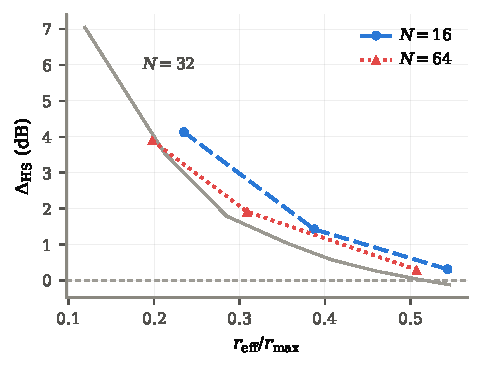
\includegraphics[width=0.92\columnwidth]{fig/fig7_boundary_invariance.pdf}
\caption{HS-GS gain against the normalized effective rank
$\rho=\reff/\rmax$ for $N\in\{16,32,64\}$. The gain approaches zero in a similar
region of $\rho$ for the three array sizes. Only the $N=32$ crossing is
bracketed by measurements of both signs; the other two are extrapolated past
the last measured cell, and the $N=16$ curve sits above the $N=64$ curve at
every matched $\rho$ by $0.49$~dB on average.}
\label{fig:rho}
\end{figure}

We also carried out a test to see what happens when the channel becomes more
complex and the low-rank constraint starts to become harmful. In this test the
Cadzow step was forced to remain active, so the estimator was denied the option
of declining to constrain. This is a diagnostic and not the proposed method.
% src: results/p12/B2_forced.json, N16_L14 row: delta_forced_active_db,
% ci_forced_active, abstention_rate.
At $\rho=0.735$, the gain becomes $-0.075$~dB with a $95\%$ interval of
$[-0.186,-0.026]$~dB, which excludes zero. Forcing a low-rank constraint on a
complex channel therefore does measurable harm, not merely no good.

At that same operating point the unforced estimator declines to constrain on
$38.8\%$ of trials. Selecting the full rank is what protects it, and on this
evidence that protection is worth having. It remains a property of the
operator rather than a property of the selection rule: these measurements show
that abstention is available and that it is used often here, not that it is
chosen whenever it should be.

\subsubsection{Is $\rho$ actually the right descriptor?}

Up to this point we have shown that $\rho$ organises the results. We have not
shown that it organises them better than something simpler, and those are
different claims. An earlier version of this paper made the second claim
without testing it. This subsection tests it.

We compare three candidate descriptors, each used in exactly the same way: the
path count $L$, the normalized path count $L/\rmax$, and $\rho=\reff/\rmax$.
The prediction rule is piecewise-linear interpolation on a fixed eight-point
table, with no regression and no curve fitting. The table is the $N=32$
path-count sweep, and the same eight rows are used for all three descriptors;
only the horizontal coordinate changes. We then predict six cells at $N=16$ and
$N=64$ that are not in the table, and compare against what was measured there.

% src: reports/p22/p32_score.json and p32_score_secondary.json; prediction rule
% verified to reproduce the 1.30 and 0.648 dB predictions quoted later in this
% section. Pre-registered in reports/p22/PREREG_P32.md before scoring.
\begin{center}
\footnotesize
\begin{tabular}{lccc}
\toprule
Descriptor & Mean error (dB) & Worst (dB) & Sign correct \\
\midrule
$L$ & 1.91 & 2.85 & 5 of 6 \\
$L/\rmax$ & \textbf{0.34} & 1.06 & \textbf{6 of 6} \\
$\rho=\reff/\rmax$ & 0.46 & 1.61 & 5 of 6 \\
\bottomrule
\end{tabular}
\end{center}

The result is clear in one direction and negative in the other.

\textbf{Normalizing by array capacity is what matters.} Raw path count is a
poor predictor across array sizes, with a mean error of $1.91$~dB, and it could
not be otherwise: $L=7$ is close to the ceiling when $\rmax=8$ and far below it
when $\rmax=32$, so the same $L$ describes opposite situations. Dividing by
$\rmax$ removes that problem and cuts the error by more than a factor of five.

\textbf{The effective rank buys nothing beyond that.} $\rho$ is not better than
the much simpler $L/\rmax$; it is slightly worse on both mean error and sign
agreement. The difference between them is not resolved by six cells --- the
paired interval on the difference is $[-0.16,+0.40]$~dB and includes zero ---
so the honest statement is that this evidence does not separate them, and
certainly does not favour $\rho$. Repeating the comparison on the wider
SNR~$\ge5$~dB summary gives the same ordering, $0.56$~dB for $L/\rmax$ against
$0.61$~dB for $\rho$.

We therefore do not claim that effective rank describes this behaviour better
than path count does. What the experiments support is narrower: \emph{path
count normalized by the array's structural capacity} predicts when the
constraint helps, and $\rho$ is one way of performing that normalization which
this evidence does not distinguish from the simpler one. We continue to use
$\rho$ in this paper because it extends naturally to channels whose paths have
unequal strengths, where $L$ is ambiguous --- but that is a reason of
convenience, and we report it as one.

Two limits apply to $\rho$ whichever way it is read. It does not determine the
size of the improvement, since the gain still changes with array size at
matched $\rho$. And it is computed from the true noiseless channel, which the
receiver does not have, so it explains the simulation results rather than
serving as a quantity an estimator could evaluate before estimating.

\subsection{Evaluation on Different Channel Distributions}

So far, the relationship between $\rho$ and the HS-GS gain has been obtained
from our original channel simulations. We now test whether this relationship is
still useful when the paths are generated differently.

The idea of this test is simple. We first use the relationship already obtained
between $\rho$ and the HS-GS gain to make a prediction. We then generate
channels using a different distribution, run HS-GS, and compare the measured
gain with the prediction. The previously obtained relationship is not changed
using the new results.

For example, the first test uses a clustered Saleh--Valenzuela channel. In this
model, propagation paths occur in clusters instead of being generated in the
same way as in the original simulations. For this channel distribution, the
normalized effective rank is
\begin{equation}
\rho=0.331.
\end{equation}

From the previously obtained relationship, this value of $\rho$ predicts an
HS-GS gain of
\begin{equation}
\Delta_{\mathrm{HS}}=1.30~\mathrm{dB}.
\end{equation}

After running 276 trials, the measured gain is 1.173~dB, with a $95\%$
confidence interval of $[1.017,1.380]$~dB. Therefore, the difference between
the predicted and measured gains is only 0.13~dB.

% [NEW] The draft did not say what the second distribution was. A reader cannot
% judge a generalisation test without knowing what it generalised to.
A second channel distribution is tested in the same way. This one uses a fixed
number of $L=10$ paths for every user, with gains drawn as
$\alpha_\ell\sim\CN(0,1)$ and angles drawn uniformly on
$(-90^\circ,90^\circ)$, following the receive-side channel configuration
of~\cite{precoding2408}. It is therefore quite different from the first test:
the clustered model groups its paths together, while this one spreads ten
independent paths across the whole angular range. In this case,
\begin{equation}
\rho=0.400.
\end{equation}

The predicted gain is 0.648~dB. After 266 trials, the measured gain is
0.963~dB, with a $95\%$ confidence interval of $[0.808,1.086]$~dB. The
prediction error is 0.315~dB.

The two results are summarized below.

\begin{center}
\footnotesize
\begin{tabular}{cccc}
\toprule
$\rho$ & Predicted gain & Measured gain & Error \\
\midrule
$0.331$ & $1.30$ dB & $1.173$ dB & $0.13$ dB \\
$0.400$ & $0.648$ dB & $0.963$ dB & $0.315$ dB \\
\bottomrule
\end{tabular}
\end{center}

The second prediction is noticeably less accurate than the first, and it falls
outside the confidence interval of the measured gain. That interval describes
the uncertainty of the measurement and not the uncertainty of the prediction,
so this is not a formal rejection of the relationship. It does mean we should
not describe the agreement as close in both cases. The honest summary is that
the relationship places an unseen channel distribution on the correct part of
the curve, and that it is not accurate to a tenth of a decibel in general.

These results are important because the new channel distributions were not used
to obtain the original relationship between $\rho$ and the HS-GS gain. The
relationship still gives reasonably close predictions when the path
distributions are changed.

However, these tests do not use a completely different channel model. Both new
channel distributions still follow the geometric channel model in
\eqref{eq:chan}. What changes is how the path numbers, path strengths, and path
angles are generated. Therefore, these results show that the relationship can
extend across different multipath distributions within the channel model
considered in this work.

\subsection{Additional Results}

We also look at how the number of users affects the results and whether it has
a large effect on the benefit of HS-GS. We test
\begin{equation}
K\in\{2,3,4\}.
\end{equation}

For SNR values of 5~dB and above, the HS-GS gain changes by only 0.094~dB
across these three cases. Therefore, within the range tested, changing the
number of users has only a small effect on the improvement provided by the
Hankel constraint.

We also examine the computational cost of HS-GS. The main extra cost comes from
choosing the Hankel rank. This rank-selection step accounts for $57.7$--$85.5\%$
of the total run-time.

\subsection{Where the Structural Step is Applied}
\label{sec:placement}

Finally we test whether the Cadzow step needs to be applied during the EM-GS
iterations at all. The two estimators being compared are HS-GS as defined
above, which applies the step after every update, and a cheaper alternative
that runs EM-GS to its full budget and then applies one Cadzow step to the
result. Both use the same selected rank on each trial, so the comparison
isolates placement and nothing else.

% src: results/p22/p22_d1_placement.json, 300 paired trials per SNR,
% configuration A; reproduces results/p12/B5.json exactly.
We had registered in advance that applying the step during the iteration would
be worth $0.3$ to $1.5$~dB. \textbf{It is not.} Averaged over the six SNR
values the difference is $+0.003$~dB, and an interval over those six points,
$[-0.12,+0.12]$~dB, contains zero comfortably. The registered prediction
failed.

\begin{center}
\footnotesize
\begin{tabular}{crcc}
\toprule
SNR (dB) & Interleaved $-$ post-hoc (dB) & 95\% CI & Median $q$ \\
\midrule
$-5$ & $-0.081$ & $[-0.159,+0.047]$ & 0.546 \\
$0$ & $-0.164$ & $[-0.317,-0.066]$ & 0.266 \\
$5$ & $+0.034$ & $[-0.050,+0.133]$ & 0.134 \\
$10$ & $+0.010$ & $[-0.071,+0.077]$ & 0.071 \\
$15$ & $+0.054$ & $[-0.014,+0.107]$ & 0.040 \\
$20$ & $+0.168$ & $[+0.102,+0.246]$ & 0.022 \\
\bottomrule
\end{tabular}
\end{center}

\textbf{That average hides a sign change.} Interleaving is significantly
\emph{worse} at $0$~dB and significantly \emph{better} at $20$~dB, and the two
effects are of similar size. The mean is near zero because they cancel, not
because nothing is happening. Reporting only the mean would have been
reporting the cancellation.

\textbf{The two estimators are not producing the same estimate.} A difference
of means cannot tell us whether two methods agree, because two different
estimates can have the same error. So we also measured, on each trial, how far
apart the two estimates are:
\begin{equation}
q_i=\frac{\bigl\|\hat\bG_i^{\text{interleaved}}
-\hat\bG_i^{\text{post-hoc}}\bigr\|_F}{\|\bG_i\|_F},
\label{eq:qdiv}
\end{equation}
which expresses the gap between them as a fraction of the channel being
estimated. The last column of the table gives the median. At $-5$~dB the two
estimates differ by $55\%$ of the channel norm while their errors differ by
$0.08$~dB. At $0$~dB they differ by $27\%$ while their errors differ by
$0.16$~dB. Even at $20$~dB, where the agreement is closest, the gap is $2.2\%$.

So the honest conclusion is narrower than ``placement does not matter''. On
this evidence the two placements are \emph{equally accurate on average while
being visibly different estimators}, and the difference between them shrinks as
the SNR rises. Because the post-hoc version is also much cheaper --- one Cadzow
step instead of $T$ of them --- it is the better practical choice here, and we
say so even though it is not the variant this paper proposes. What we cannot
say is that the two are interchangeable: they are not the same estimate, they
differ in opposite directions at the ends of the SNR range, and a single
averaged number conceals both facts.

\section{Limitations and Conclusion}

This work studies when low-rank Hankel structure can help magnitude-only
channel estimation for Rydberg atomic receivers.

The main point is easy to understand. The Hankel constraint is useful when the
channel is simple compared with the rank that the Hankel matrix can support.
For example, a channel that only needs a few important components has more
low-rank structure that can be used during estimation. As the channel becomes
more complex and uses most of the available rank, the benefit becomes smaller.
If a low-rank constraint is forced on a channel that is too complex, it can
eventually make the estimate worse.

The experiments first show this using the number of propagation paths. At
$N=32$, the HS-GS gain decreases from 7.04~dB when $L=2$ to $-0.12$~dB when
$L=16$. However, the number of paths alone is not a complete measure of channel
complexity because some paths can be much weaker than others.

What the experiments support is that path count must be measured \emph{relative
to the array's structural capacity}. Raw path count does not transfer between
array sizes, because $L=7$ is near the ceiling when $\rmax=8$ and far below it
when $\rmax=32$. In a held-out test on six cells at $N=16$ and $N=64$,
predicting from raw $L$ gives a mean error of $1.91$~dB, while predicting from
the normalized count $L/\rmax$ gives $0.34$~dB.

We use the normalized effective rank
\begin{equation}
\rho=\frac{\reff}{\rmax}
\end{equation}
as our normalization throughout, because it extends to channels whose paths
have unequal strengths, where counting paths is ambiguous. On the same held-out
test it scores $0.46$~dB, which is not better than the simpler $L/\rmax$ and
not separated from it by six cells. \textbf{We therefore do not claim that
effective rank describes this behaviour better than path count does}; the
claim we make is about normalizing by capacity, and $\rho$ is one way to do it.

For $N=16$, 32, and 64, the HS-GS gain approaches zero at $\rho=0.588$, 0.518,
and 0.544, so a factor of four in array size leaves the crossing in the same
region. Two of those three values are extrapolated rather than bracketed by
measurements of both signs, and the $N=16$ curve sits about $0.49$~dB above the
$N=64$ curve at every matched $\rho$, so this is a similar region and not a
coincident one. In the cases tested here, the Hankel constraint is most useful
when the channel effectively uses about half or less of the available Hankel
rank.

The relationship is also examined using two additional channel distributions
that were not used to build it. The predicted HS-GS gains differ from the
measured gains by 0.13 and 0.315~dB.

\textbf{Limitations.} All results in this work are obtained from simulations.
We have not yet tested the method using measured hardware data or recorded
Rydberg channels. The additional channel distributions also still follow the
geometric ULA model in \eqref{eq:chan}. Therefore, the results do not show that
the same behaviour will hold when the actual channel does not follow this
model.

The results also apply only to the magnitude-only Rydberg architecture
described in Section~II. A superheterodyne Rydberg receiver recovers both
amplitude and phase, and the problem studied here does not arise for it.

Another limitation is that $\rho$ is calculated using the true noiseless
channel in our simulations. The receiver does not know this channel in
practice. Therefore, $\rho$ is currently used to explain when the method works
rather than as a value that the receiver can calculate before channel
estimation.

The Cadzow step used here is a denoising step and not a projection, as shown in
Section~\ref{sec:estimator}. It is also a weaker requirement than the array model itself, so
a result about this constraint is not automatically a result about the physical
multipath model.

Finally, although the point where the HS-GS gain approaches zero is similar
across the tested array sizes, the exact amount of gain does not perfectly
follow $\rho$. Therefore, $\rho$ helps explain the useful region of the Hankel
constraint, but it does not completely predict its performance in every case.
The CRLB and CCRB are also used only as theoretical reference curves, because
the estimators considered here are not assumed to be unbiased and because we do
not give enough detail for those curves to be independently reproduced.

\begin{thebibliography}{99}

\bibitem{cui2025} M.~Cui, Q.~Zeng, and K.~Huang, ``Towards atomic MIMO
receivers,'' \emph{IEEE J. Sel. Areas Commun.}, vol.~43, no.~3, pp.~659--673,
2025.

\bibitem{gong2025mag} T.~Gong \emph{et al.}, ``Rydberg atomic quantum receivers
for classical wireless communication and sensing,'' \emph{IEEE Wireless
Commun.}, vol.~32, no.~5, pp.~90--100, 2025.

\bibitem{gerchberg1972} R.~W.~Gerchberg and W.~O.~Saxton, ``A practical
algorithm for the determination of phase from image and diffraction plane
pictures,'' \emph{Optik}, vol.~35, pp.~237--246, 1972.

% Order follows first appearance in the text (IEEE style): xu2025 is cited
% before xiao2026 in the introduction, so it comes first here.
\bibitem{xu2025} B.~Xu, J.~Zhang, Z.~Chen, B.~Cheng, Z.~Liu, Y.-C.~Wu, and
B.~Ai, ``Channel estimation for Rydberg atomic receivers,'' \emph{IEEE Wireless
Commun. Lett.}, vol.~14, no.~9, pp.~2957--2961, 2025.

\bibitem{xiao2026} J.~Xiao, J.~Wang, M.~Zeng, H.~Xu, X.~Li, and
A.~Nallanathan, ``Channel estimation for Rydberg atomic quantum receivers:
unrolled phase retrieval from holographic snapshots,'' \emph{IEEE Signal
Process. Lett.}, vol.~33, pp.~1696--1700, 2026.

\bibitem{balan2015} R.~Balan, ``The Fisher information matrix and the
Cram\'er--Rao bound in a non-AWGN model for the phase retrieval problem,'' in
\emph{Proc. Int. Conf. Sampling Theory Appl. (SampTA)}, 2015.

\bibitem{chen2014emac} Y.~Chen and Y.~Chi, ``Robust spectral compressed sensing
via structured matrix completion,'' \emph{IEEE Trans. Inf. Theory}, vol.~60,
no.~10, pp.~6576--6601, 2014.

\bibitem{jin2016aloha} K.~H.~Jin, D.~Lee, and J.~C.~Ye, ``A general framework
for compressed sensing and parallel MRI using annihilating filter based
low-rank Hankel matrix,'' \emph{IEEE Trans. Comput. Imag.}, vol.~2, no.~4,
pp.~480--495, 2016.

\bibitem{haldar2014} J.~P.~Haldar, ``Low-rank modeling of local $k$-space
neighborhoods (LORAKS) for constrained MRI,'' \emph{IEEE Trans. Med. Imag.},
vol.~33, no.~3, pp.~668--681, 2014.

\bibitem{tang2013} G.~Tang, B.~N.~Bhaskar, P.~Shah, and B.~Recht, ``Compressed
sensing off the grid,'' \emph{IEEE Trans. Inf. Theory}, vol.~59, no.~11,
pp.~7465--7490, 2013.

\bibitem{cadzow1988} J.~A.~Cadzow, ``Signal enhancement---a composite property
mapping algorithm,'' \emph{IEEE Trans. Acoust., Speech, Signal Process.},
vol.~36, no.~1, pp.~49--62, 1988.

\bibitem{markovsky2008} I.~Markovsky, ``Structured low-rank approximation and
its applications,'' \emph{Automatica}, vol.~44, no.~4, pp.~891--909, 2008.

\bibitem{royvetterli2007} O.~Roy and M.~Vetterli, ``The effective rank: a
measure of effective dimensionality,'' in \emph{Proc. Eur. Signal Process.
Conf. (EUSIPCO)}, 2007, pp.~606--610.

% Title and arXiv identifier confirmed by the author. The author list is taken
% from paper/master/refs.bib and has NOT been verified against the paper; see
% docs/open-todos.md item 6.3.
\bibitem{precoding2408} M.~Cui, Q.~Zeng, and K.~Huang, ``MIMO precoding for
Rydberg atomic receivers,'' 2024, arXiv:2408.14366.

\bibitem{gorman1990} J.~D.~Gorman and A.~O.~Hero, ``Lower bounds for parametric
estimation with constraints,'' \emph{IEEE Trans. Inf. Theory}, vol.~36, no.~6,
pp.~1285--1301, 1990.

\bibitem{stoica1998} P.~Stoica and B.~C.~Ng, ``On the Cram\'er--Rao bound under
parametric constraints,'' \emph{IEEE Signal Process. Lett.}, vol.~5, no.~7,
pp.~177--179, 1998.

\end{thebibliography}

\end{document}
